\chapter{Perancangan}
\label{chap:Perancangan}

Pada bab 4 dibahas mengenai perancangan aplikasi mulai dari diagram \textit{sequence}, diagram kelas secara rinci, deskripsi artibut dan \textit{method} dari setiap kelas, dan perancangan antarmuka.

%Perancangan Diagram Sequence
\section{Diagram \textit{Sequence}}
\label{lab:Diagram Sequence}
\hspace{0.5cm} Diagram \textit{sequence} merupakan diagram yang menggambarkan interaksi antar objek dalam suatu skenario. Gambar diagram \textit{sequence} dapat dilihat pada gambar ~\ref{fig:sequence lokasi perangkat} sampai ~\ref{fig:sequence rute}. 

% Sequence mendapat lokasi perangkat
\begin{figure}[h]
	\centering
		\includegraphics[scale=0.4]{Gambar/sequence/MendapatkanKordinatPerangkat}
	\caption{Diagram \textit{sequence} Mendapatkan Kordinat Perangkat}
	\label{fig:sequence lokasi perangkat}
\end{figure}

\hspace{0.5cm} Diagram ~\ref{fig:sequence lokasi perangkat} merupakan diagram \textit{sequence} untuk penentuan lokasi asal/tujuan dengan masukan lokasi perangkat. Diagram menunjukan bahwa setelah aplikasi dibuka maka aplikasi akan mencari dahulu lokasi perangkat dengan memanfaatkan kelas LocationFinder. Lalu setelah aplikasi terbuka jika pengguna ingin memilih lokasi tersebut sebagai lokasi asal maka pengguna harus menekan tombol "here". Setelah tombol "here" ditekan maka kelas MainPage akan mengambil nilai \textit{Latitude} dan nilai \textit{Longitude} dari kelas LocatonFinder. Setelah lokasi didapatkan maka aplikasi memunculkan tulisan "here" pada \textit{textbox} di kelas MainPage.

% Sequence mendapat lokasi dari peta
\begin{figure}[h]
	\centering
		\includegraphics[scale=0.4]{Gambar/sequence/MendapatkanKordinatDiMap}
	\caption{Diagram \textit{sequence} Mendapatkan Kordinat pada Peta}
	\label{fig:sequence lokasi pada peta}
\end{figure}

\hspace{0.5cm} Diagram ~\ref{fig:sequence lokasi pada peta} merupakan diagram \textit{sequence} untuk memilih lokasi. Diagram menunjukkan bahwa setelah aplikasi dibuka maka pengguna dapat menekan tombol "map". Setelah tombol "map" ditekan maka halaman akan dialihkan ke kelas Map. Saat kelas Map terbuka maka lokasi yang ditunjukan adalah lokasi dimana perangkat berada. Untuk mengetahui lokasi kelas Map mengambil kordinat \textit{latitude} dan \textit{longitude} dari kelas LocationFinder. Di kelas "Map" pengguna dapat memilih lokasi dengan memilih lokasi pada peta dan memanggil \textit{method map\_tap()}, lalu setelah pengguna memilih tempat pengguna akan menekan tombol Pilih Lokasi yang akan memanggil \textit{method pilihLokasi()}. Lokasi yang dipilih pengguna akan disimpan di kelas MainPage dan pada masukan akan tertulis "Maps". 

\hspace{0.5cm} Diagram ~\ref{fig:sequence rute} merupakan diagram \textit{sequence} untuk mencari rute. Diagram menunjukan bahwa setelah aplikasi dibuka maka aplikasi akan melakukan inisialisasi. Untuk mencari rute dari lokasi asal ke lokasi tujuan dibutuhkan kordinat \textit{latitude} lokasi asal, \textit{longitude} lokasi asal, \textit{latitude} lokasi tujuan, dan \textit{longitude} lokasi tujuan. Jika pengguna mendapatkan lokasi dari peta atau sesuai lokasi maka yang didapatkan sudah pasti koordinat, namun jika pengguna memasukkan kata kunci perlu didapat koordinat \textit{latitude} dan \textit{longitude} dari kata kunci tersebut. Jika masukan yang didapat berupa kata kunci maka akan dilakukan pemeriksaan apakah koordinat untuk kata kunci tersebut tersedia. Pemeriksaan dilakukan dengan melakukan pemanggilan Kiri API. Tahap pemanggilan meliputi pemangilan \textit{method GetStringAsync()} lalu mengjadikan objek kembaliannya dengan \textit{method Deselialize()}. Jika sudah didapat dan hasilnya lebih dari satu maka akan dipanggil \textit{method getListItem()} yang menampilkan daftar pilihan ke pengguna untuk dipilih. Pengguna dapat memilih tempat sesuai tempat asal maupun tujuan yang diinginkan. Setelah lokasi asal dan lokasi tujuan didapat maka kelas MainPage akan mengarahkan ke kelas Route untuk menampilkan hasilnya. Kelas Route akan memanggil \textit{method OnNavigatedTo()} yang bertujuan untuk mendapatkan lokasi asal dan lokasi tujuan. Pada kelas Route, kelas Route akan memanggil \textit{method Find()} lalu mengembalikan rute yang ditemukan kepada pengguna.

% Sequence mendapat rute
\begin{figure}[h!]
	\centering
		\includegraphics[scale=0.35]{Gambar/sequence/MendapatkanRute}
	\caption{Diagram \textit{sequence} Mendapatkan Rute}
	\label{fig:sequence rute}
\end{figure}

\newpage

%Perancangan Kelas
\section{Perancangan Kelas}
\label{lab:Perancangan Kelas}
\hspace{0.5cm} Pada sub-bab ini dibahas mengenai deskripsi kelas secara rinci pada aplikasi Pencari Rute Kendaraan Umum untuk Windows Phone. Untuk lebih jelas mengenai kelas yang ada pada aplikasi ini, penyajian gambar diagram kelas yang dapat dilihat pada  gambar ~\ref{fig:kelas}. 

% Kelas tanpa atribut 
\begin{figure}[h!]
	\centering
		\includegraphics[scale=0.5]{Gambar/useCase_dan_Class/class4kosong}
	\caption{Diagram Kelas}
	\label{fig:kelas}
\end{figure}

%Kelas diagram rinci per kelas
Berikut penjelasan kelas diagram secara rinci dengan setiap kelas disertai atribut dan \textit{method}.

% Kelas
\begin{figure}[h!]
	\centering
		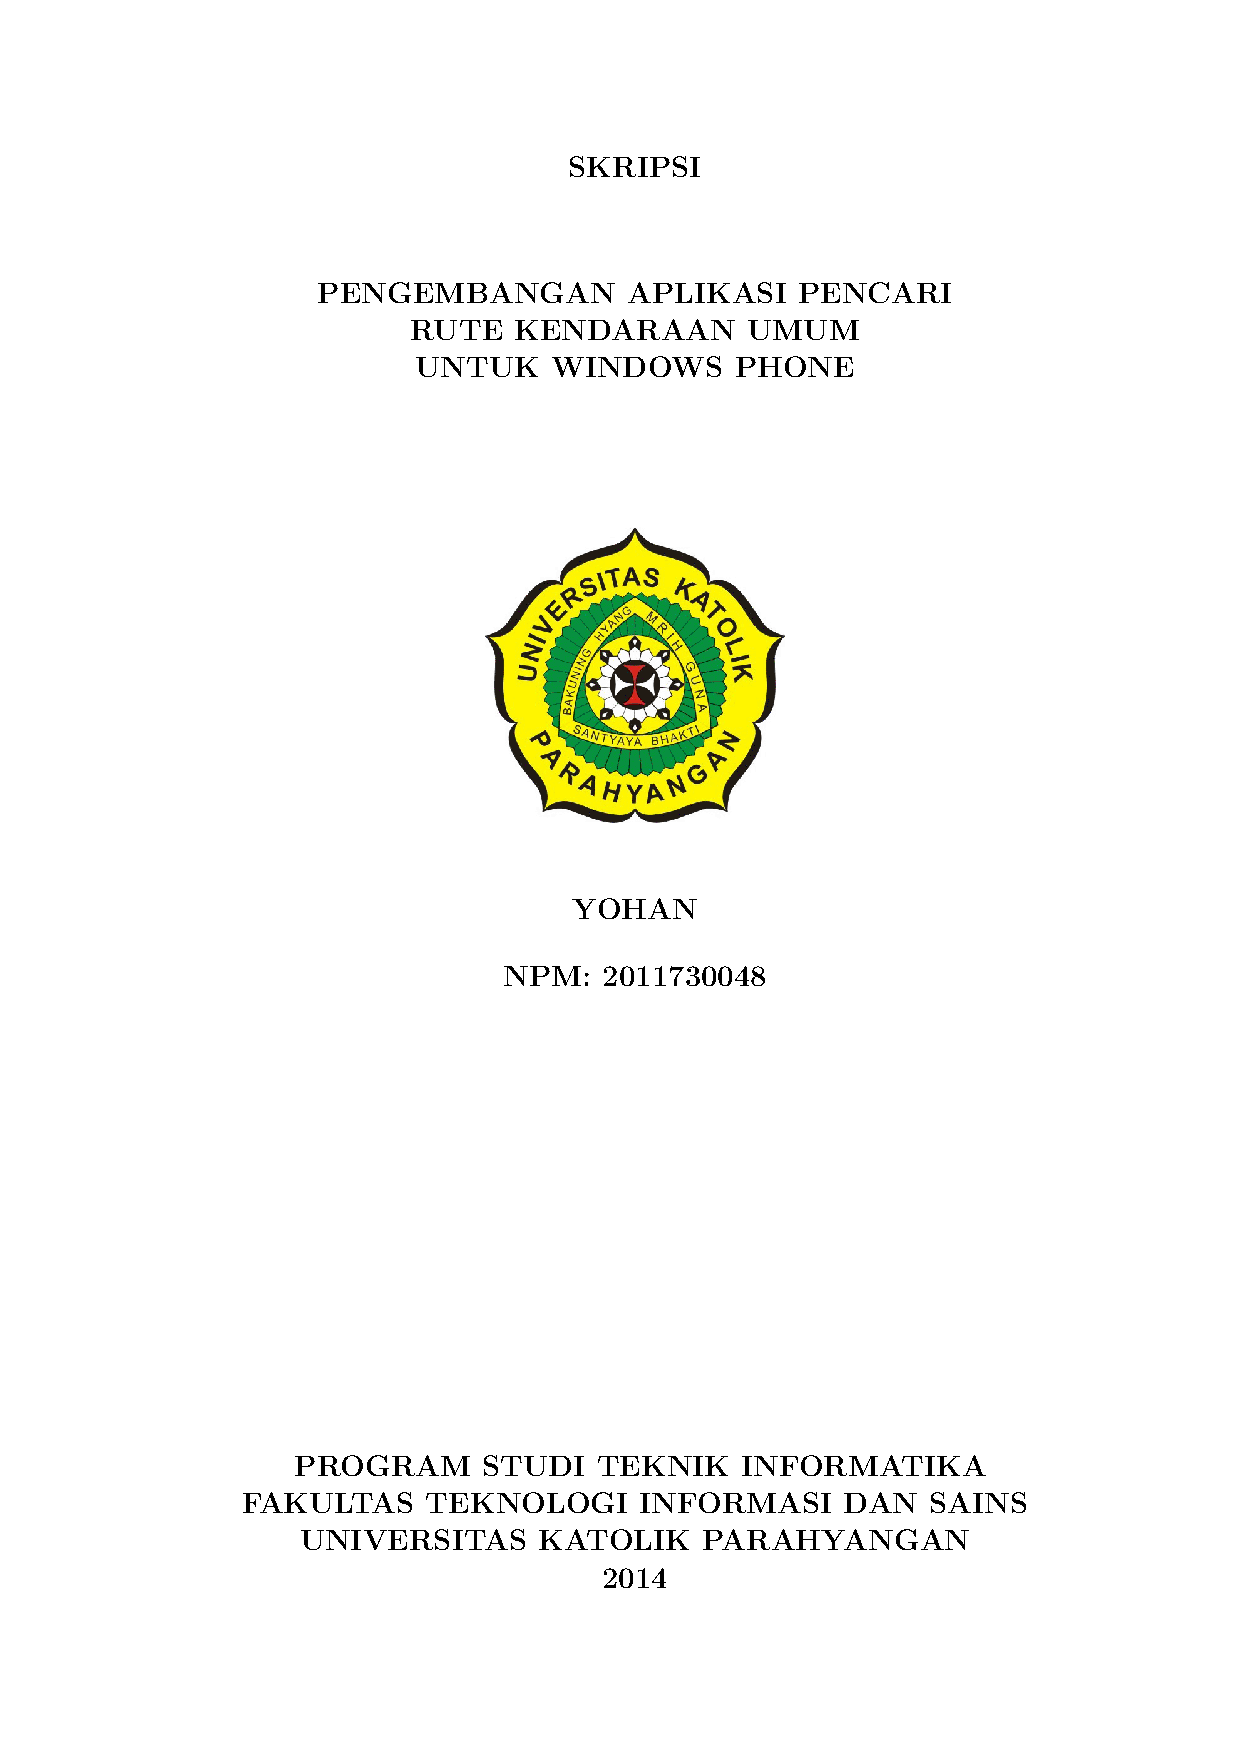
\includegraphics[scale=0.6]{Gambar/useCase_dan_Class/perClass/main}
	\caption{Kelas Mainpage (sub-bab ~\ref{lab:Kelas PhoneApplicationPage})}
	\label{fig:kelasMainpage}
\end{figure}

% Kelas
\begin{figure}[h!]
	\centering
		\includegraphics[scale=0.7]{Gambar/useCase_dan_Class/perClass/city}
	\caption{Kelas City (sub-bab ~\ref{lab:Kelas City})}
	\label{fig:kelasCity}
\end{figure}

% Kelas
\begin{figure}[h!]
	\centering
		\includegraphics[scale=0.7]{Gambar/useCase_dan_Class/perClass/jsonConvert}
	\caption{Kelas JsonConvert (sub-bab ~\ref{lab:Kelas JsonConvert})}
	\label{fig:kelasJsonConvert}
\end{figure}

% Kelas
\begin{figure}[h!]
	\centering
		\includegraphics[scale=0.7]{Gambar/useCase_dan_Class/perClass/locationFinder}
	\caption{Kelas LocationFinder (sub-bab ~\ref{lab:Kelas LocationFinder})}
	\label{fig:kelaslLocationFinder}
\end{figure}

% Kelas
\begin{figure}[h!]
	\centering
		\includegraphics[scale=0.7]{Gambar/useCase_dan_Class/perClass/map}
	\caption{Kelas Map (sub-bab ~\ref{lab:Kelas PhoneApplicationPage})}
	\label{fig:kelaslMap}
\end{figure}

% Kelas
\begin{figure}[h!]
	\centering
		\includegraphics[scale=0.6]{Gambar/useCase_dan_Class/perClass/packageWindowsPhone}
	\caption{\textit{Package} WindowsPhone (sub-bab ~\ref{lab:Kelas BackgroundWorker} sampai ~\ref{lab:Kelas Geoposition})}
	\label{fig:kelaslPackageWindowsPhone}
\end{figure}

\newpage

% Kelas
\begin{figure}[h!]
	\centering
		\includegraphics[scale=0.7]{Gambar/useCase_dan_Class/perClass/protocol}
	\caption{Kelas Protocol (sub-bab ~\ref{lab:Kelas Protocol})}
	\label{fig:kelaslProtocol}
\end{figure}

% Kelas
\begin{figure}[h!]
	\centering
		\includegraphics[scale=0.7]{Gambar/useCase_dan_Class/perClass/route}
	\caption{Kelas Route (sub-bab ~\ref{lab:Kelas Route})}
	\label{fig:kelaslRoute}
\end{figure}

% Kelas
\begin{figure}[h!]
	\centering
		\includegraphics[scale=0.7]{Gambar/useCase_dan_Class/perClass/SearchPlace}
	\caption{Kelas SearchPlace (sub-bab ~\ref{lab:Kelas RootObjectSearchPlace} dan ~\ref{lab:Kelas SearchResult})}
	\label{fig:kelaslSearchPlace}
\end{figure}

% Kelas
\begin{figure}[h!]
	\centering
		\includegraphics[scale=0.7]{Gambar/useCase_dan_Class/perClass/FindRoute}
	\caption{Kelas FindRoute (sub-bab ~\ref{lab:Kelas RootObjectFindRoute} dan ~\ref{lab:Kelas RoutingResult})}
	\label{fig:kelasFindRoute}
\end{figure}

\clearpage
%Kelas PhoneApplicationPage
\subsection{Kelas \textit{PhoneApplicationPage}}
\label{lab:Kelas PhoneApplicationPage}
\hspace{0.5cm} \textit{PhoneApplicationPage} merupakan kelas bawaan Windows Phone yang menangani interaksi pengguna dengan aplikasi dan siklus hidup aplikasi.

%Kelas MainPage
\subsection{Kelas \textit{MainPage}}
\label{lab:Kelas MainPage}
\hspace{0.5cm} \textit{MainPage} merupakan kelas turunan dari kelas \textit{PhoneApplicationPage} yang menangani interaksi langsung antara halaman aplikasi dengan pengguna. Pada kelas ini ditaruh kontrol yang diperlukan. Berikut adalah penjelasan atribut-atribut yang dimiliki kelas ini:
\begin{enumerate}
	\item protocol bertipe Protocol untuk mendapatkan URL yang digunakan dalam permintaan ke Kiri API.
	\item lFinder bertipe LocationFinder digunakan untuk menampung semua informasi mengenai lokasi.
	\item httpClient bertipe HttpClient merupakan objek yang digunakan untuk mengurus permintaan dan kembalian dari Kiri API.
	\item city bertipe kumpulan String untuk menampung kota yang didukung oleh layanan Kiri.
	\item myCity bertipe String untuk menampung kode kota sesuai Kode Penerbangan IATA.
	\item backgroundWorker bertipe BackgroundWorker untuk mengurus pencarian lokasi di belakang layar.
\end{enumerate}

Berikut adalah penjelasan beberapa \textit{method} yang dimiliki kelas ini:
\begin{enumerate}
	\item Konstruktor MainPage digunakan untuk memuat komponen yang ada di halaman MainPage dan mendapatkan kota terdekat dari lokasi perangkat.
	\item \textit{method} OnNavigatedTo digunakan untuk mendapatkan lokasi dari peta dan mendapatkan objek LocationFinder. \textit{Method} ini secara otomatis dipanggil jika pengguna kembali ke kelas MainPage. \textit{Method} ini memiliki parameter NavigationEventArgs.
	\item \textit{Method} Application\_Deactivated digunakan untuk menyimpan \textit{state} objek saat meninggalkan aplikasi. \textit{method} ini memiliki parameter object dan DeactivatedEventArgs.
	\item \textit{Method} Application\_Activated digunakan untuk mengambil \textit{state} objek saat kembali ke aplikasi. \textit{method} ini memiliki parameter object dan ActivatedEventArgs.
	\item \textit{Method} startRoute digunakan untuk mendapatkan masukan pengguna. Jika masukan didapat dari peta atau lokasi perangkat berarti sudah dalam kordinat, namun jika masukan didapat dari \textit{query} maka akan dicari lokasi yang terkait sesuai \textit{query} tersebut. Lokasi terkait yang didapatkan lalu dikembalikan ke pengguna untuk dipilih. Setelah pengguna lokasi dalam bentuk kordinat didapatkan maka kelas akan diarahkan ke kelas Route. \textit{method} ini memiliki parameter objek tombol dan event.
	\item \textit{Method} changeMapFrom digunakan untuk berpindah ke halaman mapFrom. \textit{Method} ini memiliki parameter objek tombol dan event.
	\item \textit{Method} changeMapTo digunakan untuk berpindah ke halaman mapTo. \textit{method} ini memiliki parameter objek tombol dan event.
	\item \textit{Method} getHereFrom digunakan untuk mendapatkan kordinat perangkat lalu menyimpan nilainya di kordinat asal di kelas LocationFinder dan menulisakan "Here" pada \textit{TextBox} lokasi asal. \textit{Method} ini memiliki parameter objek tombol dan event.
	\item \textit{Method} getHereTo digunakan untuk mendapatkan kordinat perangkat lalu menyimpan nilainya di kordinat tujuan di kelas LocationFinder dan menulisakan "Here" pada \textit{TextBox} lokasi tujuan. \textit{Method} ini memiliki parameter objek tombol dan event.
	\item \textit{Method} getListItem digunakan untuk membuat \textit{listBox} lalu menampilkan ke pengguna. \textit{method} ini memiliki parameter RootObjectSearchPlace dan string yang menunjukan \textit{list} yang ditampilkan untuk lokasi asal dan lokasi tujuan. 
	\item \textit{Method} ListBoxSelectedPlace digunakan untuk mendapatkan tempat asal yang dipilih pengguna. \textit{method} ini memiliki parameter objek dan \textit{event SelectionChangedEventArgs}. 
	\item \textit{Method} searchCoordinatePlace digunakan untuk mencari kordinat dari tempat pilihan pengguna. \textit{method} ini memiliki parameter \textit{ListBox} dan tempat yang dipilih dalam bentuk \textit{string}.
	\item \textit{Method} findRoute digunakan untuk berpindah ke kelas Route jika lokasi asal dan lokasi tujuan sudah ditentukan.
	\item \textit{Method} changeCity digunakan untuk mengubah kota tujuan dari pencarian. \textit{method} ini memiliki parameter objek dan \textit{event SelectionChangedEventArgs}.
	\item \textit{Method} showCity digunakan untuk mencari kota yang paling dekat dengan lokasi perangkat.
	\item \textit{Method} ShowSplash digunakan untuk menampilkan tampilan awal untuk proses inisialisasi aplikasi.
	\item \textit{Method} StartLoadingData digunakan untuk memanggil BackgroundWorker. BackgroundWorker digunakan untuk melakukan aksi di belakang layar.
	\item \textit{Method} backgroundWorker\_DoWork digunakan untuk melakukan pemanggilan aksi di belakang layar. \textit{method} ini memiliki parameter objek dan DoWorkEventArgs.
	\item \textit{Method} backgroundWorker\_RunWorkerCompleted digunakan untuk melakukan pemanggilan saat BackgroundWorker selesai melakukan tugasnya. \textit{method} ini memiliki parameter objek dan \textit{RunWorkerCompletedEventArgs}.
\end{enumerate}

%Kelas City
\subsection{Kelas \textit{City}}
\label{lab:Kelas City}
\hspace{0.5cm} \textit{City} merupakan kelas yang menyimpan kota-kota yang mendukung pencarian rute kendaraam umum dengan bantuan Kiri. Berikut adalah penjelasan atribut-atribut yang dimiliki kelas ini:
\begin{enumerate}
	\item centerCity bertipe \textit{array of GeoCoordinate} untuk menyimpan kordinat pusat dari kota.
	\item city bertipe \textit{array of String} untuk menyimpan nama kota.
	\item cityCode bertipe \textit{array of String} untuk menyimpan kode kota dalam huruf kecil sesuai aturan IATA Airport Code. 
\end{enumerate}

Berikut adalah penjelasan beberapa \textit{method} yang dimiliki kelas ini:
\begin{enumerate}
	\item Konstruktor City digunakan untuk untuk inisialisasi nilai atribut.
	\item \textit{Method} getNearby digunakan untuk mencari kota terdekat dengan lokasi perangkat. \textit{method} ini mengembalikan interger yang merupakan index kota pada atribut city. \textit{method} ini memiliki 2 buah parameter yaitu \textit{latitude} dan \textit{longitude} yang bertipe \textit{double}.
	\item \textit{Method} getIndexFromCityCode digunakan untuk mencari indeks pada \textit{array}  sesuai kode kota. \textit{method} ini memiliki parameter bertipe \textit{string} yang merupakan kode kota.
\end{enumerate}

%Kelas BackgroundWorker
\subsection{Kelas \textit{BackgroundWorker}}
\label{lab:Kelas BackgroundWorker}
\hspace{0.5cm} \textit{BackgroundWorker} merupakan kelas yang dipakai untuk mengeksekusi operasi pada \textit{thread} terpisah. Berikut adalah penjelasan \textit{event} yang dimiliki kelas ini dan dipakai untuk perancangan aplikasi:
\begin{enumerate}
	\item \textit{Event} DoWork
	\item \textit{Event} RunWorkerCompleted
\end{enumerate}
Berikut adalah penjelasan beberapa \textit{method} yang dimiliki kelas ini:
\begin{enumerate}
	\item \textit{Method} RunWorkerAsync() digunakan untuk memulai operasi di belakang layar.
\end{enumerate}

%Kelas Geocoordinate
\subsection{Kelas \textit{Geocoordinate}}
\label{lab:Kelas Geocoordinate}
\hspace{0.5cm} \textit{Geocoordinate} merupakan kelas bawaan dari Windows Phone yang dimanfaatkan untuk membaca \textit{latitude} dan \textit{longitude}.

%Kelas Geolocator
\subsection{Kelas \textit{Geolocator}}
\label{lab:Kelas Geolocator}
\hspace{0.5cm} \textit{Geolocator} merupakan kelas bawaan Windows Phone untuk mengkases lokasi. Dengan bantuan kelas ini maka dapat mengetahui status lokasi dari perangkat dan menemukan lokasi secara akurat.

%Kelas Geoposition
\subsection{Kelas \textit{Geoposition}}
\label{lab:Kelas Geoposition}
\hspace{0.5cm} \textit{Geoposition} merupakan kelas yang menampung lokasi sesuai kembalian \textit{Geolocator}.

%Kelas LocationFinder
\subsection{Kelas \textit{LocationFinder}}
\label{lab:Kelas LocationFinder}
\hspace{0.5cm} \textit{LocationFinder} merupakan kelas yang menampung lokasi dan pencarian lokasi. Berikut adalah penjelasan atribut-atribut yang dimiliki kelas ini:
\begin{enumerate}
	\item coorLat bertipe Double untuk menampung kordinat latitude pengguna.
	\item coorLong bertipe Double untuk menampung kordinat longitude pengguna.
	\item coorLatFrom bertipe Double untuk menampung kordinat latitude lokasi asal yang diinginkan pengguna.
	\item coorLongFrom bertipe Double untuk menampung kordinat longitude lokasi asal yang diinginkan pengguna.
	\item coorLatTo bertipe Double untuk menampung kordinat latitude lokasi tujuan yang diinginkan pengguna.
	\item coorLongTo bertipe Double untuk menampung kordinat longitude lokasi tujuan yang diinginkan pengguna.
	
	\item addressDevice bertipe String untuk menyimpan alamat perangkat berada.
	\item addressDeviceFrom bertipe String untuk menyimpan alamat berdasarkan lokasi lokasi asal yang diinginkan pengguna.
	\item addressDeviceTo bertipe String untuk menyimpan alamat berdasarkan lokasi tujuan yang diinginkan pengguna.
	
	\item geolocator bertipe Geolocator untuk menampung pengaturan mendapatkan lokasi.
	\item myReverseGeocodeQuery bertipe ReverseGeocodeQuery untuk konversi dari alamat ke lokasi dan sebalikny.
	\item myCoordinate bertipe GeoCoordinate untuk menampung kordinat geografis.
	\item accuracy bertipe double untuk menampung akurasi perangkat mendapatkan lokasi.
\end{enumerate}

Berikut adalah penjelasan beberapa \textit{method} yang dimiliki kelas ini:
\begin{enumerate}
	\item Konstruktor LocationFinder berfungsi mengatur atribut geolocator dan mencari lokasi perangkat.
	\item \textit{Method} findLocation berfungsi inisialisasi GPS lalu mendapat kordinat dan menampungnya di atribut.
	\item \textit{Method} updateAccuracy berfungsi untuk mengubah nilai akurasi dari perangkat.
	\item \textit{Method} setPositionChanged berfungsi mengubah atribut coorLat, atribut coorLong, dan akurasi jika terdapat perubahan lokasi. \textit{method} ini memiliki parameter Geolocator dan PositionChangedEventArgs yang akan menjalankan \textit{method} jika terdapat perubahan yang diberitahukan melalui kelas Geolocator.
	\item \textit{Method} GetCurrentCoordinate berfungsi mengubah posisi saat ini, posisi lokasi asal, dan lokasi tujuan. \textit{method} ini memiliki tiga buah parameter \textit{latitude} bertipe Double, \textit{longitude} bertipe Double, dan paramFor bertipe String. Parameter \textit{latitude} dan \textit{longitude} merupakan lokasi sedangkan parameter paramFor digunakan sebagai tujuan perubahan lokasi. 
	\item \textit{Method} ReverseGeocodeQueryFrom\_QueryCompleted berfungsi untuk mencari alamat lokasi asal. \textit{method} ini memiliki parameter objek dan QueryCompletedEventArgs< IList<MapLocation> >.
	\item \textit{Method} ReverseGeocodeQueryTo\_QueryCompleted berfungsi untuk mencari alamat lokasi tujuan. \textit{method} ini memiliki parameter objek dan QueryCompletedEventArgs< IList<MapLocation> >.
	\item \textit{Method} ReverseGeocodeQuery\_QueryCompleted berfungsi untuk mencari alamat lokasi perangkat. \textit{method} ini memiliki parameter objek dan QueryCompletedEventArgs< IList<MapLocation> >.
	\item \textit{Method} setCoordinateHere berfungsi untuk menyimpan kordinat dan alamat perangkat ke kordinat dan alamat lokasi asal dan lokasi tujuan. \textit{Method} ini memiliki parameter paramFor bertipe \textit{string} yang digunakan sebagai masukan disimpannya lokasi perangkat.
	\item \textit{Method} reset berfungsi untuk memasang kembali lokasi asal dan lokasi tujuan.
\end{enumerate}

%Kelas Map
\subsection{Kelas \textit{Map}}
\label{lab:Kelas Map}
\hspace{0.5cm} \textit{Map} merupakan kelas yang digunakan untuk mendapatkan titik yang ditunjuk pengguna pada peta lalu menerjemahkannya dalam bentuk titik kordinat. Berikut adalah penjelasan atribut-atribut yang dimiliki kelas ini:
\begin{enumerate}
	\item lFinder bertipe LocationFinder digunakan untuk menampung semua informasi mengenai lokasi.
	\item fromMapFor bertipe string digunakan sebagai indikator lokasi asal atau lokasi tujuan yang didapatkan dari map.
\end{enumerate}

Berikut adalah penjelasan beberapa \textit{method} yang dimiliki kelas ini:
\begin{enumerate}
	\item Konstruktor Map untuk inisialisasi dan penambahan \textit{event} mengetuk pada peta.
	\item \textit{Method} OnNavigatedTo berfungsi untuk mendapatkan masukan lokasi asal atau lokasi tujuan yang ditentukan dari map untuk kemudian ditampung di objek LocationFinder. \textit{method} ini memiliki sebuah parameter NavigationEventArgs.
	\item \textit{Method} OnNavigatedFrom digunakan untuk mengirimkan \textit{state} objek LocationFinder saat berpindah kelas. \textit{method} ini memiliki parameter NavigationEventArgs.
	\item \textit{Method} ShowMyLocationOnTheMap digunakan untuk memberitahu dan menandai lokasi perangkat.
	\item \textit{Method} map\_Tap berfungsi untuk menandai lokasi yang ditunjuk pengguna lalu  menerjemahkan lokasi yang ditunjuk pengguna pada peta dan mengirimnya ke kelas LocationFinder.
	\item \textit{Method} pilihLokasi berfungsi berpindah ke kelas MainPage dan memberitahu kelas MainPage bahwa lokasi sudah dipilih. \textit{method} ini memiliki parameter objek tombol dan \textit{event}.
\end{enumerate}

%Kelas HttpClient
\subsection{Kelas \textit{HttpClient}}
\label{lab:Kelas HttpClient}
\hspace{0.5cm} \textit{HttpClient} merupakan kelas bawaan Windows Phone untuk mengatur pengiriman dan kembalian menggunakan protokol HTTP. Berikut adalah penjelasan \textit{method} kelas \textit{HttpClient} yang dipakai untuk perancangan aplikasi ini:
\begin{enumerate}
	\item \textit{Method} GetStringAsync membutuhkan parameter alamat bertipe \textit{string} dan mengembalikan kembalian dari Kiri dalam bentuk \textit{Task<string>}.
\end{enumerate}

%Kelas JsonConvert
\subsection{Kelas \textit{JsonConvert}}
\label{lab:Kelas JsonConvert}
\hspace{0.5cm} \textit{JsonConvert} merupakan kelas yang menyediakan \textit{method} untuk mengkonversi berbagai jenis komponen \textit{common language runtime} dan \textit{JSON}. Kelas ini merupakan bagian \textit{namespace Newtonsoft}.  Berikut adalah penjelasan \textit{method} yang dipakai untuk perancangan aplikasi:
\begin{enumerate}
	\item \textit{Method} DeserializeObject berfungsi untuk konversi dari bentuk \textit{string} menjadi objek. \textit{Method} ini memiliki satu parameter bertipe \textit{string} lalu mengembalikan \textit{string} tersebut dalam bentuk objek.
\end{enumerate}

%Kelas Protocol
\subsection{Kelas \textit{Protocol}}
\label{lab:Kelas Protocol}
\hspace{0.5cm} \textit{Protocol} merupakan kelas untuk menampung semua alamat dalam pengiriman menggunakan protokol HTTP. Berikut adalah penjelasan atribut-atribut yang dimiliki kelas ini:
\begin{enumerate}
	\item uri\_version bertipe \textit{string} digunakan untuk menyimpan nama dari parameter uri.
	\item uri\_mode bertipe \textit{string} digunakan untuk menyimpan nama dari parameter mode.
	\item uri\_locale bertipe \textit{string} digunakan untuk menyimpan nama dari parameter locale.
	\item uri\_start bertipe \textit{string} digunakan untuk menyimpan nama dari parameter start.
	\item uri\_finish bertipe \textit{string} digunakan untuk menyimpan nama dari parameter finish.
	\item uri\_presentation bertipe \textit{string} digunakan untuk menyimpan nama dari parameter presentation.
	\item uri\_apikey bertipe \textit{string} digunakan untuk menyimpan nama dari parameter apikey.
	\item uri\_region bertipe \textit{string} digunakan untuk menyimpan nama dari parameter region.
	\item uri\_query bertipe \textit{string} digunakan untuk menyimpan nama dari parameter query.

	\item apiKey bertipe \textit{string} digunakan untuk menyimpan nilai kunci API untuk mengirim permintaan ke Kiri.
	\item hostname bertipe \textit{string} digunakan untuk digunakan untuk menyimpan alamat host dari Kiri.
	\item handle bertipe \textit{string} digunakan untuk menyimpan alamat host ditambah "handle.php".
	\item iconPath bertipe \textit{string} digunakan untuk menyimpan lokasi gambar yang dibutuhkan.
	\item iconStart bertipe \textit{string} digunakan untuk menyimpan lokasi gambar awal perjalanan dari lokasi awal.
	\item iconFinish bertipe \textit{string} digunakan untuk menyimpan lokasi gambar akhir perjalanan ke lokasi tujuan.
	
	\item version\_2 bertipe \textit{string} digunakan untuk menyimpan nilai versi dari API yang digunakan (saat pembuatan penelitian ini versi Kiri API yang digunakan adalah versi 2).
	\item modeFind bertipe \textit{string} yang digunakan untuk menyimpan nilai "searchplace" yang merupakan mode mencari lokasi terkait pada Kiri API.
	\item modeRoute bertipe \textit{string} yang digunakan untuk menyimpan nilai "findroute" yang merupakan mode mencari rute pada Kiri API.
	\item modeNearby bertipe \textit{string} yang digunakan untuk menyimpan nilai "nearbytransport	" yang merupakan mode mencari lokasi terdekat pada Kiri API.
	
	\item localeId bertipe \textit{string} yang digunakan untuk menyimpan nilai bahasa jika kembalian yang diinginkan ingin berbahasa Indonesia.
	\item localeEn bertipe \textit{string} yang digunakan untuk menyimpan nilai bahasa jika kembalian yang diinginkan ingin berbahasa Inggris.
	\item presentationMobile bertipe \textit{string} yang digunakan untuk menyimpan nilai penyajian untuk perangkat \textit{mobile}.
	\item presentationDesktop bertipe \textit{string} yang digunakan untuk menyimpan nilai penyajian untuk perangkat \textit{desktop}.
\end{enumerate}

Berikut adalah penjelasan beberapa \textit{method} yang dimiliki kelas ini:
\begin{enumerate}
	\item \textit{Method} getTypeTransport merupakan \textit{method} yang akan mengembalikan alamat dari gambar transportasi dengan bingkai. \textit{Method} ini memiliki 2 parmeter yaitu means sebagai tipe transportasi dan meansDetail sebagai nama kendaraan.
	\item \textit{Method} getTypeTransportWOBaloon merupakan \textit{method} yang mengembalikan alamat dari gambar transportasi tanpa bingkai tambahan. \textit{Method} ini memiliki 2 parmeter yaitu means sebagai tipe transportasi dan meansDetail sebagai nama kendaraan.
	\item \textit{Method} getSearchPlace merupakan \textit{method} yang mengembalikan URI pencarian lokasi sesuai paramater. Parameter yang dimaksud adalah kata kunci masukan pengguna.
	\item \textit{method} getFindRoute merupakan \textit{method} yang mengembalikan URI pencarian rute sesuai parameter. Parameter yang dimaksud adalah kordinat lokasi asal dan kordinat lokasi tujuan yang bertipe \textit{string}.
	\item \textit{Method} getRequestSearch digunakan untuk mendapatkan lokasi terkait sesuai masukan pengguna. \textit{Method} ini mengembalikan Task<RootObjectSearchPlace> karena menggunakan operasi \textit{asynchronous}. \textit{Method} ini memiliki parameter kata kunci masukan pengguna dan kota yang masing-masing parameter bertipe \textit{string}.
		\item \textit{Method} getRequestRoute digunakan untuk mendapatkan rute sesuai lokasi asal dan lokasi tujuan. \textit{Method} ini mengembalikan Task<RootObjectFindRoute> karena menggunakan operasi \textit{asynchronous}. \textit{method} ini memiliki parameter \textit{latitude} lokasi asal, \textit{longitude} lokasi asal, \textit{latitude} lokasi tujuan, dan \textit{longitude} lokasi tujuan yang masing-masing bertipe \textit{double}.
\end{enumerate}

%Kelas RootObjectSearchPlace
\subsection{Kelas \textit{RootObjectSearchPlace}}
\label{lab:Kelas RootObjectSearchPlace}
\hspace{0.5cm} \textit{RootObjectSearchPlace} merupakan kelas untuk menampung objek hasil pencarian lokasi. Berikut adalah penjelasan atribut-atribut yang dimiliki kelas ini:
\begin{enumerate}
	\item status bertipe string digunakan untuk menampung hasil kembalian status dari Kiri.
	\item searchresult bertipe \textit{list} dan menampung banyak objek SearchResult. 
	\item attributions bertipe objek untuk menampung \textit{attributions}.
\end{enumerate}


%Kelas SearchResult
\subsection{Kelas \textit{SearchResult}}
\label{lab:Kelas SearchResult}
\hspace{0.5cm} \textit{SearchResult} merupakan kelas untuk menampung nama tempat dan kordinat dari nama tempat tersebut. Berikut adalah penjelasan atribut-atribut yang dimiliki kelas ini:
\begin{enumerate}
	\item placename bertipe \textit{string} digunakan untuk menampung nama tempat. 
	\item location bertipe \textit{string} digunakan untuk menampung nama tempat.
\end{enumerate}

%Kelas RootObjectFindRoute
\subsection{Kelas \textit{RootObjectFindRoute}}
\label{lab:Kelas RootObjectFindRoute}
\hspace{0.5cm} \textit{RootObjectFindRoute} merupakan kelas untuk menampung hasil pencarian rute. Berikut adalah penjelasan atribut-atribut yang dimiliki kelas ini:
\begin{enumerate}
	\item status bertipe \textit{string} digunakan untuk menampung hasil kembalian status dari Kiri.
	\item routingresults bertipe \textit{list} dan menampung banyak objek RoutingResult.
\end{enumerate}

%Kelas RoutingResult
\subsection{Kelas \textit{RoutingResult}}
\label{lab:Kelas RoutingResult}
\hspace{0.5cm} \textit{RoutingResult} merupakan kelas untuk menampung langkah menuju tempat tujuan dan waktu yang dibutuhkan. Berikut adalah penjelasan atribut-atribut yang dimiliki kelas ini:
\begin{enumerate}
	\item steps bertipe \textit{list} digunakan untuk menampung tiap langkah dari lokasi asal ke lokasi tujuan. Tiap langkah yang dimaksud adalah kendaraan yang digunakan, jalur yang dilewati, dan informasi yang dibutuhkan pengguna.
	\item traveltime bertipe \textit{string} digunakan untuk menampung waktu yang dibutuhkan dari lokasi asal ke lokasi tujuan.
\end{enumerate}

%Kelas Route
\subsection{Kelas \textit{Route}}
\label{lab:Kelas Route}
\hspace{0.5cm} \textit{Route} merupakan kelas untuk pencarian rute dan menampilkannya kepada pengguna. Berikut adalah penjelasan atribut-atribut yang dimiliki kelas ini:
\begin{enumerate}
	\item listBoxStatus bertipe \textit{boolean} digunakan untuk menentukan nilai status rute dalam bentuk daftar sedang tertutup(bernilai \textit{false}) atau terbuka(bernilai \textit{true}). 
	\item lFinder bertipe LocationFinder digunakan untuk menampung semua informasi mengenai lokasi.
	\item arrayFocus bertipe \textit{array of Point} digunakan untuk menampung titik fokus perubahan jenis transportasi yang digunakan pengguna.  
	\item detailRoute bertipe \textit{array of String} digunakan untuk menampung keterangan yang dibutuhkan pengguna dari Kiri API.
	\item focusPointNumber bertipe \textit{integer} digunakan untuk menentukan \textit{index of} dari atribut arrayFocus dan detailRoute.
	\item routeLayer bertipe MapLayer digunakan untuk menampung \textit{Polyline} dan \textit{Pushpin}
	\item myLocationLayer bertipe MapLayer digunakan untuk menampung titik dari lokasi perangakt berada.
	\item p bertipe Protocol digunakan untuk menampung permintaan data dengan Kiri API.
	\item geolocator bertipe Geolocator untuk menangani perubahan lokasi yang terjadi.
	\item newTimer bertipe DispatcherTimer digunakan untuk membuat perngatur waktu.
	\item timeOut bertipe boolean digunakan untuk menentukan nilai status apakah waktu untuk satu proses sudah mencapai batas.
	\item backgroundWorker bertipe BackgroundWorker digunakan untuk menangain proses di belakang layar.
\end{enumerate}

Berikut adalah penjelasan beberapa \textit{method} yang dimiliki kelas ini:
\begin{enumerate}
	\item Konstruktor Route digunakan untuk memuat komponen yang ada di halaman Route, inisialisasi atribu, dan pemanggilan backgroundWorker.
	\item \textit{Method} OnNavigatedTo digunakan untuk mendapatkan objek LocationFinder dan memanggil \textit{method} TrackLocation. \textit{method} ini memiliki parameter NavigationEventArgs.
	\item \textit{Method} OnNavigatedFrom digunakan untuk mengirimkan \textit{state} objek LocationFinder saat berpindah kelas. \textit{method} ini memiliki parameter NavigationEventArgs.
	\item \textit{Method} Application\_Deactivated digunakan untuk menyimpan \textit{state} objek saat meninggalkan aplikasi. \textit{method} ini memiliki parameter object dan DeactivatedEventArgs.
	\item \textit{Method} TrackLocation digunakan untuk inisislisasi GeoLocator dan dan memulai pelacakan lokasi terus menerus. 
	\item \textit{Method} geolocator\_StatusChanged digunakan untuk mengetahui status GeoLocator.
	\item \textit{Method} geolocator\_PositionChanged digunakan untuk mengetahui perubahan lokasi yang terjadi dan menyimpannya di kelas LocationFinder.
	\item \textit{Method} Find digunakan untuk mencari rute yang dicari pengguna.
	\item \textit{Method} setRouteToMap digunakan untuk menggambar rute dan lokasi pada \textit{layer} peta. \textit{method} ini memiliki parameter RootObjectFindRoute yang merupakan objek untuk pencarian rute.
	\item \textit{Method} setFocus digunakan untuk mengarahkan pusat pandangan ke titik lokasi pergantian jenis transportasi. \textit{method} ini memiliki parameter objek dan RoutedEventArgs.
	\item \textit{Method} toMyLocation digunakan untuk mengarahkan pusat pandangan ke titik lokasi perangakt berada. \textit{method} ini memiliki parameter objek dan RoutedEventArgs.
	\item \textit{Method} ShowList digunakan untuk membuka dan menutup rute dalam bentuk daftar. \textit{method} ini memiliki parameter objek dan RoutedEventArgs.
	\item \textit{Method} createNew digunakan untuk membuat objek Pushpins. \textit{method} ini memiliki parameter uri bertipe String, transport bertipe String yang menandakan jenis transportasi, dan geoCoordinate bertipe GeoCoordinate sebagai lokasi dari Pushpins.
	\item \textit{Method} drawMyLocationOnTheMap digunakan untuk membuat penanda lokasi di lapisan myLocationLayer pada peta. \textit{method} ini memiliki parameter latitude bertipe double dan longitude bertipe double.
	\item \textit{Method} back digunakan untuk konfirmasi ke pengguna jika pengguna ingin meninggalkan aplikasi. \textit{method} ini memiliki dua buah parameter sender bertipe objek dan e bertipe RoutedEventArgs.
	\item \textit{Method} ShowLoading digunakan untuk memunculkan \textit{popup} menunggu.
	\item \textit{Method} StartLoadingData digunakan untuk pemanggilan BackgroundWorker.
	\item \textit{Method} backgroundWorker\_DoWork digunakan untuk eksekusi \textit{method} dengan BackgroundWorker. \textit{method} ini memiliki dua buah parameter sender bertipe objek dan e bertipe DoWorkEventArgs.
	\item \textit{Method} backgroundWorker\_RunWorkerCompleted digunakan untuk menutup \textit{popup} menunggu jika semua \textit{method} sudah selesai dijalankan. \textit{method} ini memiliki dua buah parameter sender bertipe objek dan e bertipe RunWorkerCompletedEventArgs.
	\item \textit{Method} OnBackKeyPress digunakan untuk konfirmasi ke pengguna jika pengguna ingin meninggalkan aplikasi dengan menekan tombol "back". \textit{method} ini memiliki parameter e bertipe CancelEventArgs.
\end{enumerate}

%Perancangan Antar Muka
\section{Perancangan Antar Muka}
\label{lab:Perancangan Kelas}
\hspace{0.5cm} Pada sub-bab ini dibahas mengenai antarmuka pada aplikasi Pencari Rute Kendaraan Umum untuk Windows Phone. Antarmuka berfungsi sebagai jembatan yang menghubungkan antara aplikasi dengan pengguna. Berikut ini dijelaskan mengenai rancangan antarmuka aplikasi Pencari Rute Kendaraan Umum untuk Windows Phone. 

%Kelas MainPage
\subsection{Antarmuka Kelas MainPage}
\label{lab:Antarmuka Kelas MainPage}

% Antarmuka Main
\begin{figure}[h]
	\centering
		\includegraphics[scale=0.6]{Gambar/perancangan_antarmuka/Home}
	\caption{Antarmuka \textit{MainPage}}
	\label{fig:Antarmuka MainPage}
\end{figure}

\hspace{0.5cm} Antarmuka Kelas Map pada gambar ~\ref{fig:Antarmuka MainPage} merupakan tampilan awal saat aplikasi dijalankan. Antarmuka Kelas Map memiliki dua buah masukan, lima buah tombol, dan satu menu daftar. Berikut adalah detailnya.

Dua buah masukan yaitu.
\begin{itemize}
	\item Masukan lokasi asal\\
	Merupakan masukan lokasi asal mula pengguna ingin melakukan perjalanan.
	\item Masukan lokasi tujuan\\
	Merupakan masukan lokasi tujuan berhentinya perjalanan.
\end{itemize}

Lima buah tombol yaitu. 
\begin{itemize}
	\item Tombol map untuk lokasi asal\\
	Jika tombol ditekan maka halaman akan berpindah ke kelas map untuk memilih lokasi asal di peta. Jika di kelas Map pengguna memilih lokasi maka pada masukan lokasi asal terdapat tulisan "Maps".
	\item Tombol here untuk lokasi asal\\
	Jika tombol ditekan maka lokasi asal adalah lokasi perangkat saat tombol ditekan dan masukan lokasi asal menjadi "here".
	\item Tombol map untuk lokasi tujuan\\
	Jika tombol ditekan maka halaman akan berpindah ke kelas map untuk memilih lokasi tujuan di peta. Jika di kelas Map pengguna memilih lokasi maka pada masukan lokasi tujuan terdapat tulisan "Maps".
	\item Tombol here untuk lokasi tujuan\\
	Jika tombol ditekan maka lokasi tujuan adalah lokasi perangkat saat tombol ditekan dan masukan lokasi tujuan menjadi "here".
	\item Tombol find\\
	Jika tombol ditekan maka aplikasi akan menampilkan daftar tempat asal dan tempat tujuan lalu mengarahkan ke Kelas Route.
\end{itemize}

Satu buah daftar yaitu.
\begin{itemize}
	\item Daftar kota yang tersedia\\
	Merupakan daftar kota yang tersedia (kota yang rute angkutan umumnya dapat ditemukan dengan aplikasi ini). Disaat aplikasi dijalankan maka daftar akan menunjuk ke kota terdekat tempat perangkat berada.
\end{itemize}

%Antarmuka list Tempat
\begin{figure}[h]
	\centering
		\includegraphics[scale=0.6]{Gambar/perancangan_antarmuka/ListTempat}
	\caption{Antarmuka Daftar Tempat}
	\label{fig:Antarmuka Daftar Tempat}
\end{figure}

\hspace{0.5cm} Antarmuka Daftar Tempat pada gambar ~\ref{fig:Antarmuka Daftar Tempat} merupakan daftar yang dimunculkan jika pengguna memasukan kata kunci pada pencarian tempat asal dan tempat tujuan. Daftar akan muncul jika didapat kembalian hasil pencarian lebih dari satu.

%Kelas Map
\subsection{Antarmuka Kelas Map}
\label{lab:Antarmuka Kelas Map}

% Antarmuka Map
\begin{figure}[h]
	\centering
		\includegraphics[scale=0.6]{Gambar/perancangan_antarmuka/Map}
	\caption{Antarmuka \textit{Map}}
	\label{fig:Antarmuka Map}
\end{figure}

\hspace{0.5cm} Antarmuka Kelas Map pada gambar ~\ref{fig:Antarmuka Map} merupakan antarmuka yang menunjuk lokasi pada peta. Terdapat satu buah tombol yang dimunculkan jika pengguna sudah memilih lokasi. Jika tombol ditekan maka kordinat lokasi akan di simpan dan dikirim pada kelas MainPage dan halaman akan diarahkan ke kelas MainPage.

%Kelas Route
\subsection{Antarmuka Kelas Route}
\label{lab:Antarmuka Kelas Route}

% Antarmuka route
\begin{figure}[h]
	\centering
		\includegraphics[scale=0.6]{Gambar/perancangan_antarmuka/Route}
	\caption{Antarmuka \textit{Route}}
	\label{fig:Antarmuka Route}
\end{figure}

\hspace{0.5cm} Antarmuka Kelas Route pada gambar ~\ref{fig:Antarmuka Route} merupakan antarmuka untuk melihat rute dari lokasi asal ke lokasi tujuan dalam bentuk daftar maupun peta. Terdapat empat buah tombol pada antarmuka Kelas Route. Berikut tombol yang terdapat pada Kelas Route. 
\begin{itemize}
	\item Tombol prev\\
	Jika tombol ditekan maka akan menunjuk titik sebelumnya pada rute peta.
	\item Tombol next\\
	Jika tombol ditekan maka akan menunjuk titik setelahnya pada rute peta.
	\item Tombol here\\
	Jika tombol ditekan maka akan menunjuk lokasi perangkat berada pada peta.
	\item Tombol Show List\\
	Jika tombol ditekan maka akan menunjuk atau menyembunyikan daftar rute.
\end{itemize}

% Antarmuka list route
\begin{figure}[h]
	\centering
		\includegraphics[scale=0.6]{Gambar/perancangan_antarmuka/ListRoute}
	\caption{Antarmuka Rute dalam Bentuk Daftar}
	\label{fig:Antarmuka listRoute}
\end{figure}

\hspace{0.5cm} Antarmuka rute dalam bentuk daftar pada gambar ~\ref{fig:Antarmuka listRoute} merupakan antarmuka untuk melihat rute secara lebih jelas dengan keterangan tahap demi tahap disertai jarak dan waktu perjalanan. Antarmuka daftar dapat dilihat atau disembunyikan sesuai keinginan pengguna namun saat kelas Rute dibuka antarmuka daftar rute akan disembunyikan.